\begin{figure}[thpb]
  \centering
  %\begin{tikzpicture}
    %\clip [rounded corners=1em] (0,0) rectangle coordinate (centerpoint) (5,7.5cm);
%    \node[minimum width=\linewidth,minimum height=174pt,draw=black,rounded corners=1em,fill=bgcolor,draw=black]
%    {};
%    \node[name=img] {
      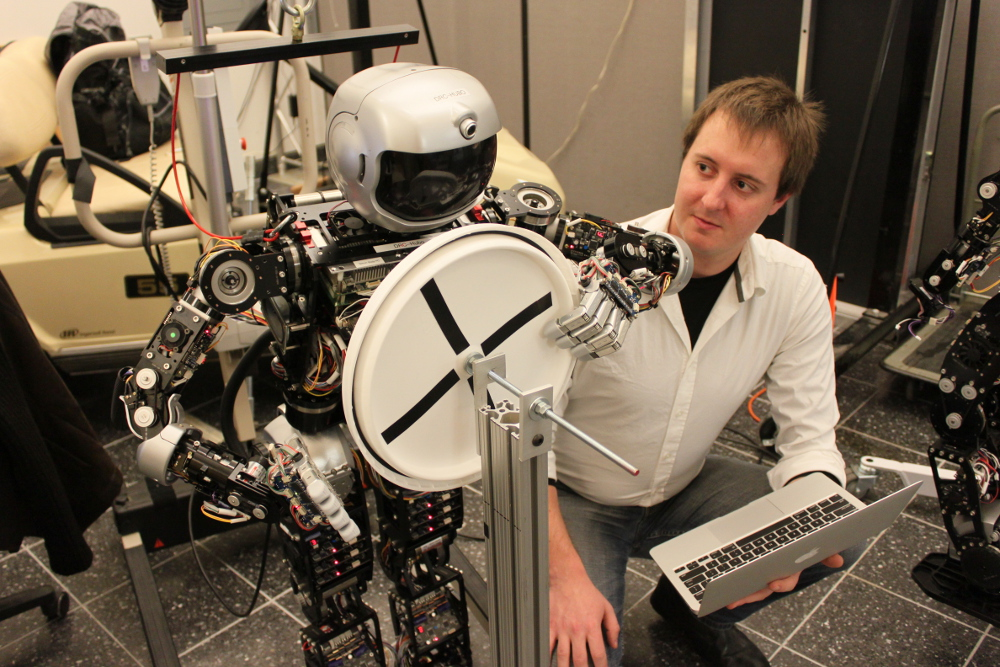
\includegraphics[width=0.93\columnwidth]{./pix/IMG_9107-small.jpg}
      
\includegraphics{./qrcode/qrcode-valve.png}\\
      Video: http://danlofaro.com/phd/valve/
%    };
%    \draw [bgcolor, rounded corners=1em, line width=1em,inner sep=0pt]
%    (img.north west) --
%    (img.north east) --
%    (img.south east) --
%    (img.south west) -- cycle
%    ;
%  \end{tikzpicture}
\caption{Hubo (left) turning a valve via Hubo-Ach alongside Daniel
  M. Lofaro (right).  Valve turning developed in conjunction with
  Dmitry Berenson at WPI for the DARPA Robotics Challenge.}
  \label{fig:valve}
\end{figure}